% verso e anverso:
% \documentclass[12pt,openright,twoside,a4paper,english]{abntex2}
% apenas verso:	
\documentclass[12pt,oneside,a4paper,english]{abntex2} 

\usepackage[alf]{abntex2cite}	% Citações padrão ABNT
\usepackage{listings}
\usepackage{float}
\usepackage{cmap}				% Mapear caracteres especiais no PDF
\usepackage{lmodern}			% Usa a fonte Latin Modern			
\usepackage[T1]{fontenc}		% Selecao de codigos de fonte.
\usepackage[utf8]{inputenc}		% Codificacao do documento (conversão automática dos acentos)
\usepackage{lastpage}			% Usado pela Ficha catalográfica
\usepackage{indentfirst}		% Indenta o primeiro parágrafo de cada seção.
\usepackage{color}				% Controle das cores
\usepackage{graphicx}			% Inclusão de gráficos
\usepackage{pdfpages}
\usepackage{tikz}
\usetikzlibrary{automata,positioning}
\usepackage{mathtools}

\definecolor{blue}{RGB}{41,5,195} % alterando o aspecto da cor azul

\makeatletter
\hypersetup{
    %pagebackref=true,
    pdftitle={\@title}, 
    pdfauthor={\@author},
    pdfsubject={\@title},
    pdfcreator={\imprimirpreambulo},
    pdfkeywords={Linguagens}{Compiladores}{Tradução dos Comandos}, 
    colorlinks=true,       		% false: boxed links; true: colored links
    linkcolor=blue,          	% color of internal links
    citecolor=blue,        		% color of links to bibliography
    filecolor=magenta,      		% color of file links
    urlcolor=blue,
    bookmarksdepth=4
}
\makeatother

\autor{Victor Lassance (6431325)}
\title{Relatório de Compiladores\\Segunda Prova\\Compilador de \emph{SimpPro} para \emph{RNA}}
\orientador[Professor:]{Ricardo Luis de Azevedo da Rocha}
\preambulo{Texto apresentado à Escola Politécnica da Universidade de São Paulo como requisito para a aprovação na disciplina Linguagens e Compiladores no quinto módulo acadêmico do curso de graduação em Engenharia de Computação, junto ao Departamento de Engenharia de Computação e Sistemas Digitais (PCS).}
\instituicao{%
	Universidade de São Paulo
	\par
	Escola Politécnica
	\par
	Engenharia de Computação - Curso Cooperativo}
\local{São Paulo}
\data{2013}
\tipotrabalho{PCS2056 - Linguagens e Compiladores}

\setlength{\parindent}{1.3cm} % O tamanho do parágrafo
\setlength{\parskip}{0.2cm}  % Controle do espaçamento entre um parágrafo e outro
\lstset{basicstyle=\footnotesize\ttfamily}
\makeindex

\begin{document}

\frenchspacing % Retira espaço extra obsoleto entre as frases.

\imprimirfolhaderosto

\tableofcontents

\textual

\chapter{Apresentação da linguagem \emph{SimpPro} e enunciado}
\label{chap:linguagem-simppro}
	% !TEX encoding = UTF-8 Unicode

A linguagem \emph{SimpPro} foi criada e apresentada pelo professor da disciplina com características similares a de outras linguagens. As principais linguagens herdadas pela \emph{SimpPro} foram de Prolog, na forma de declaração e busca; e Lisp, na utilização dos parêntesis para declarar predicados, cláusulas e a meta.

A linguagem Prolog é declarativa, o seu texto pode conter variáveis (identificáveis lexicamente) ou nomes e números (constantes) ao estilo LISP. O operador de definição de termos é “:-”, para uma verificação de meta o operador é “?-”. Um programa em Prolog é composto usualmente de três partes: conjuntos de fatos, conjuntos de cláusulas e conjuntos de metas. Os fatos são dados sobre os quais é possível efetuar uma busca por meio de unificação de literais. As cláusulas representam a forma como os elementos de dados são inter-relacionados, definem predicados, seu uso por outros predicados e a relação entre predicados e fatos. As metas definem que tipo de resultado é esperado, podendo ser um resultado booleano, um conjunto de valores possíveis para uma variável, etc. 

Para este exercício não será utilizada a linguagem Prolog completa, apenas um subconjunto bastante limitado e simplificado denominado \emph{SimpPro}. 

A sintaxe de SimpPro fornecida em BNF foi a seguinte: 

\lstinputlisting[frame=single,breaklines=true,morekeywords={not,or,eps},basicstyle=\tiny]{files/sintaxe.txt}

Considerando que a unificação é feita através de uma busca em base dados (cuja implementação é conhecida e acessível) e que haverá apenas uma meta por programa, cujo resultado será booleano, ou seja, cada programa retornará verdadeiro (1) ou falso (0) para a meta (que será uma cláusula completa), pede-se para construir um reconhecedor determinístico, baseado no autômato de pilha estruturado, que aceite como entrada válida um programa escrito em \emph{SimpPro}.

Além disso, deve-se construir o sistema de programação para a linguagem \emph{SimpPro}, que terá um compilador para a linguagem \emph{RNA} com um ambiente de execução e uma função de busca para a meta definida. Deve ser usado a implementação de \emph{RNA} feita em linguagem C para validar o código gerado pelo compilador, aceitando ou não a meta como inferência lógica dos fatos e das cláusulas. 

	
\chapter{Apresentação da linguagem \emph{RNA}}
\label{chap:linguagem-rna}
	% !TEX encoding = UTF-8 Unicode

A linguagem de programação \emph{RNA} apresentada pelo professor é uma linguagem esotérica e nunca utilizada para aplicações práticas, criada em 2008 e implementada em 2011 por Cyrus H.  

Ela possui 16 instruções implementadas e 3 variáveis para armazenamento de memória e processamento de dados, \emph{strg}, \emph{ptr} e \emph{memory}. Como a \emph{strg}, variável responsável por guardar o índice para acesso ao \emph{memory} tem 8 bits, só podemos acessar 256 células de 8 bits cada uma, tendo uma memória bem limitada.

A Figura~\ref{fig:expl-rna} mostra a relação das 3 variáveis.

\begin{figure}[htbp]
    \centering
    \includegraphics[width=0.6\textwidth]{./images/expl-rna.png}
    \caption{Ilustração das estruturas de armazenamento do \emph{RNA}.}
    \label{fig:expl-rna}
\end{figure}

As 16 instruções implementadas correspondem às seguintes instruções em C:

\begin{enumerate}
	\item \textbf{AUG}: \verb$int main() {$
	\item \textbf{UAA}: \verb$} // end_main$
	\item \textbf{UGG}: \verb$strg=0;$
	\item \textbf{AAA}: \verb$++strg;$
	\item \textbf{AAC}: \verb$--strg;$
	\item \textbf{GCA}: \verb$strg=*ptr;$
	\item \textbf{ACA}: \verb$ptr=&memory[strg];$
	\item \textbf{CCA}: \verb$scanf(“%d”, ptr);$
	\item \textbf{CUA}: \verb$printf(“%c”, *ptr);$
	\item \textbf{AGA}: \verb$*ptr+=memory[strg];$
	\item \textbf{AGC}: \verb$*ptr*=memory[strg];$
	\item \textbf{CAA}: \verb$*ptr-=memory[strg];$
	\item \textbf{CAC}: \verb$*ptr/=memory[strg];$
	\item \textbf{GAA}: \verb$*ptr=*ptr==memory[strg]?1:0;$
	\item \textbf{GAC}: \verb$while(*ptr) {$
	\item \textbf{UAC}: \verb$} // end_while$
\end{enumerate}

Com relação a implementação em C da linguagem\footnote{http://esolangs.org/wiki/RNA}, foram encontrados alguns erros que foram corrigidos a fim de permitir o teste de programas em RNA. Abaixo, segue o \emph{diff} do que foi modificado com relação à implementação original.

\lstinputlisting[frame=single,breaklines=true,basicstyle=\tiny]{files/diff_rna.txt}

A implementação do interpretador \emph{RNA} com as correções pode ser encontrada junto com o código final, para permitir a realização de testes.


\chapter{Analisador léxico}
\label{chap:lexico}
	% !TEX encoding = UTF-8 Unicode

O analisador léxico atua como uma interface entre o reconhecedor sintático, que forma, normalmente, o núcleo do compilador, e o texto de entrada, convertendo a sequência de caracteres de que este se constitui em uma sequência de átomos.

Para a consecução de seus objetivos, o analisador léxico executa usualmente uma série de funções, todas de grande importância como infraestrutura para a operação das partes do compilador mais ligadas à tradução propriamente dita do texto-fonte. As principais funções são listadas abaixo:

\begin{itemize}

	\item Extração e Classificação de Átomos;
	\begin{itemize}
		\item Principal funcionalidade do analisador;
		\item As classes de átomos mais usuais: identificadores, palavras reservadas, números inteiros sem sinal, números reais, strings, sinais de pontuação e de operação, caracteres especiais, símbolos compostos de dois ou mais caracteres especiais e comentários.
	\end{itemize}
	
	\item Eliminação de Delimitadores e Comentários;
	
	\item Conversão numérica;
	\begin{itemize}
		\item Conversão numérica de notações diversas em uma forma interna de representação para manipulação de pelos demais módulos do compilador.
	\end{itemize}
	
	\item Tratamento de Identificadores;
	\begin{itemize}
		\item Tratamento com auxílio de uma tabela de símbolos.
	\end{itemize}
	
	\item Identificação de Palavras Reservadas;
	\begin{itemize}
		\item Verificar se cada identificador reconhecido pertence a um conjunto de identificadores especiais.
	\end{itemize}
	
	\item Recuperação de Erros;
	
	\item Listagens;
	\begin{itemize}
		\item Geração de listagens do texto-fonte.
	\end{itemize}
	
	\item Geração de Tabelas de Referências Cruzadas;
	\begin{itemize}
		\item Geração de listagem indicativa dos símbolos encontrados, com menção à localização de todas as suas ocorrências no texto do programa-fonte.
	\end{itemize}
	
	\item Definição e Expansão de Macros;
	\begin{itemize}
		\item Pode ser realizado em um pré-processamento ou no analisador léxico. No caso do analisador, deve-se haver uma comunicação entres os analisadores léxico e sintático.
	\end{itemize}
	
	\item Interação com o sistema de arquivos;
	
	\item Compilação Condicional;
	
	\item Controles de Listagens.
	\begin{itemize}
		\item São os comandos que permitem ao programador que ligue e desligue opções de listagem, de coleta de símbolos em tabelas de referência cruzadas, de geração, e impressão de tais tabelas, de impressão de tabelas de símbolos do programa compilador, de tabulação e formatação das saídas impressas do programa-fonte.
	\end{itemize}

\end{itemize}

Nas próximas seções definiremos com detalhes cada um dos passos para a criação e teste do analisador léxico.


\section{Descrição do funcionamento}

O analisador léxico lê um arquivo de configuração da máquina de estados
(transdutor). O mesmo pode ser comparado à seguinte regex:

\verb!(.)([^\1]*)\1\s*([A-Za-z]+(:?_[0-9]+)?)\s*([A-Za-z]+(:?_[0-9]+)?)!

Cada linha possui uma lista de caracteres delimitados por um caractere
especial (por exemplo `+' ou `\verb!#!') e dois identificadores que designam os
estados inicial e final da transição. O caractere \verb!@! designa todas as
transições, este é usado principalmente para encaminhar qualquer aceitação
final de um sub-autômato ao estado \verb!Q0!, para então ser tratado
normalmente.

Ex:
\begin{lstlisting}
+abcdefghijklmnopqrstuvxywz+    Q0      IDENT
+ABCDEFGHIJKLMNOPQRSTUVXYWZ+    Q0      IDENT
+_+                             Q0      IDENT
\end{lstlisting}
Este exemplo vai reconhecer todos os caracteres a-z e A-Z mais o underscore
(\_) como transições do estado \verb!Q0! e \verb!IDENT!.

Após a leitura do arquivo de configuração e de um arquivo com
    \emph{keywords}, faz-se a leitura do arquivo fonte, por meio do
transdutor, percorrendo-se o arquivo fonte token a token. Uma função
\verb!next_useful_token! oferece o não retorno dos tokens de espaço, tal qual a
quebra de linha e espaços normais, além de ignorar comentários. O motor do lex também substitui classes
\verb!IDENT! para \verb!RESERVED! se a palavra se encontra na lista de
identificadores reservados. 

\section{Autômatos finitos por \emph{Token}}

\begin{itemize}

\item DELIM: \verb!/[{}()\[\];]/!

\begin{figure}[H]
	\centering
	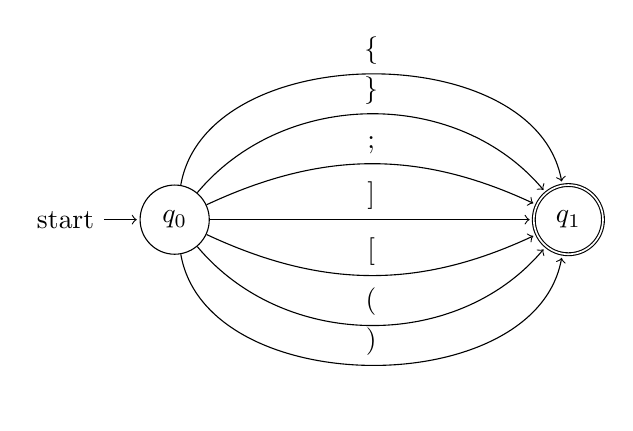
\begin{tikzpicture}[shorten >=1pt,node distance=5cm,on grid,auto] 
	   \node[state,initial] (q0)   {$q_0$}; 
	   \node[state,accepting](q1) [right=of q0] {$q_1$};
	    \path[->] 
	    (q0) edge[bend left=80]   node {\{} (q1)
	    (q0) edge[bend left=50]   node {\}} (q1)
	    (q0) edge[bend right=50]  node {(} (q1)
	    (q0) edge[bend right=80]  node {)} (q1)
	    (q0) edge[bend left=25]   node {;} (q1)
	    (q0) edge[bend right=25]  node {[} (q1)
	    (q0) edge                 node {]} (q1);
	\end{tikzpicture}
	\caption{Autômato finito DELIM}
\end{figure}

\item SPACE: \verb!/[ \t\r\n\v\f]+/!

\begin{figure}[H]
	\centering
	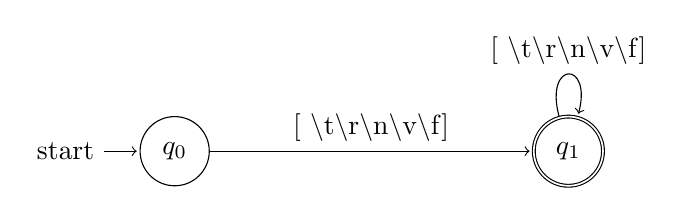
\begin{tikzpicture}[shorten >=1pt,node distance=5cm,on grid,auto] 
	   \node[state,initial] (q0)   {$q_0$}; 
	   \node[state,accepting](q1) [right=of q0] {$q_1$};
	    \path[->] 
	    (q0) edge   node {
			[ $\backslash$t$\backslash$r$\backslash$n$\backslash$v$\backslash$f]
		} (q1)
		(q1) edge[loop above]  node {
			[ $\backslash$t$\backslash$r$\backslash$n$\backslash$v$\backslash$f]
		} (q1);
	\end{tikzpicture}
	\caption{Autômato finito SPACE}
\end{figure}

\item COMMENT: \verb!/#[^\n]*/!

\begin{figure}[H]
	\centering
	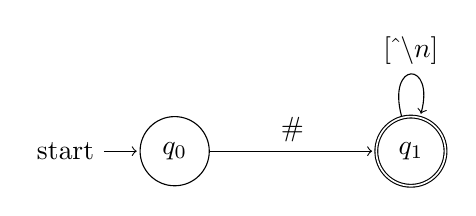
\begin{tikzpicture}[shorten >=1pt,node distance=3cm,on grid,auto] 
	   \node[state,initial] (q0)   {$q_0$}; 
	   \node[state,accepting](q1) [right=of q0] {$q_1$};
	    \path[->] 
	    (q0) edge  node {\#} (q1)
		(q1) edge[loop above]  node {$[\hat{~}\backslash n]$} (q1);
	\end{tikzpicture}
	\caption{Autômato finito COMMENT}
\end{figure}

\item IDENT: \verb!/[a-zA-Z_][a-zA-Z0-9_]*/!

\begin{figure}[H]
	\centering
	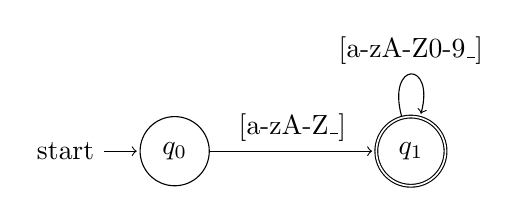
\begin{tikzpicture}[shorten >=1pt,node distance=3cm,on grid,auto] 
	   \node[state,initial] (q0)   {$q_0$}; 
	   \node[state,accepting](q1) [right=of q0] {$q_1$};
	    \path[->] 
	    (q0) edge  node {[a-zA-Z\_]} (q1)
	    (q1) edge [loop above] node {[a-zA-Z0-9\_]} (q1);
	\end{tikzpicture}
	\caption{Autômato finito IDENT}
\end{figure}

\item INTEGER: \verb!/[0-9]+/!

\begin{figure}[H]
	\centering
	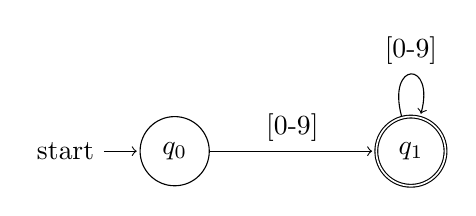
\begin{tikzpicture}[shorten >=1pt,node distance=3cm,on grid,auto] 
	   \node[state,initial] (q0)   {$q_0$}; 
	   \node[state,accepting](q1) [right=of q0] {$q_1$};
	    \path[->] 
	    (q0) edge  node {[0-9]} (q1)
	    (q1) edge [loop above] node {[0-9]} (q1);
	\end{tikzpicture}
	\caption{Autômato finito INTEGER}
\end{figure}

\item FLOAT: \verb!/[0-9]*\.[0-9]+/!

\begin{figure}[H]
	\centering
	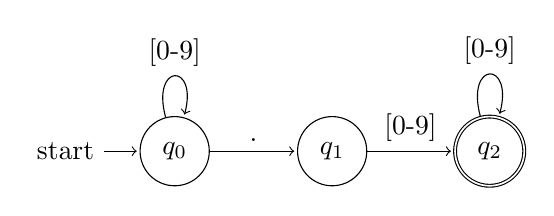
\begin{tikzpicture}[shorten >=1pt,node distance=2cm,on grid,auto] 
	   \node[state,initial] (q0)   {$q_0$}; 
	   \node[state](q1) [right=of q0] {$q_1$};
	   \node[state,accepting](q2) [right=of q1] {$q_2$};
	    \path[->] 
	    (q0) edge  node {.} (q1)
	    (q1) edge  node {[0-9]} (q2)
	    (q0) edge [loop above] node {[0-9]} (q0)
	    (q2) edge [loop above] node {[0-9]} (q2);
	\end{tikzpicture}
	\caption{Autômato finito FLOAT}
\end{figure}

\item CHAR: \verb!/'(?:\\[0abtnvfre\\'"]|[\x20-\x5B\x5D-\x7E])'/!

\begin{figure}[H]
	\centering
	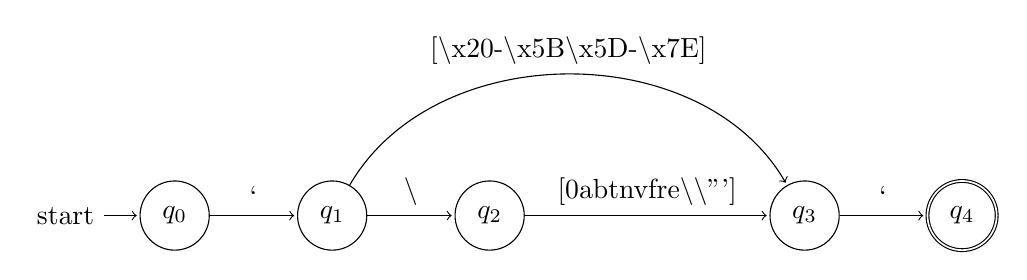
\begin{tikzpicture}[shorten >=1pt,node distance=2cm,on grid,auto] 
	   \node[state,initial] (q0)   {$q_0$}; 
	   \node[state] (q1) [right=of q0] {$q_1$}; 
	   \node[state] (q2) [right=of q1] {$q_2$}; 
	   \node[state] (q3) [right=of q2,xshift=+2cm] {$q_3$}; 
	   \node[state, accepting] (q4) [right=of q3] {$q_4$}; 
	    \path[->] 
	    (q0) edge  node {$`$} (q1)
	    (q1) edge[bend left=60] node {
	        [$\backslash$x20-$\backslash$x5B$\backslash$x5D-$\backslash$x7E]
	    } (q3)
	    (q1) edge node {$\backslash$} (q2)
	    (q2) edge node {[0abtnvfre$\backslash\backslash$"']} (q3)
	    (q3) edge node {$`$} (q4);
	\end{tikzpicture}
	\caption{Autômato finito CHAR}
\end{figure}

\item STRING: \verb!/"(?:\\"|[^"])*"/!

\begin{figure}[H]
	\centering
	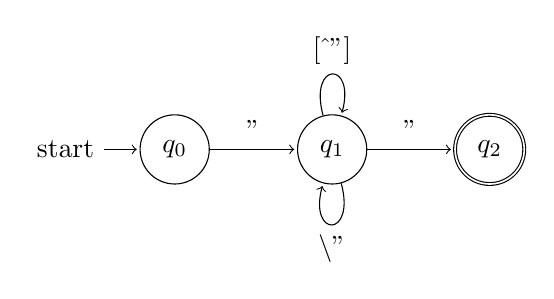
\begin{tikzpicture}[shorten >=1pt,node distance=2cm,on grid,auto] 
	   \node[state,initial] (q0)   {$q_0$}; 
	   \node[state] (q1) [right=of q0] {$q_1$}; 
	   \node[state, accepting] (q2) [right=of q1] {$q_2$}; 
	    \path[->] 
	    (q0) edge  node {$"$} (q1)
	    (q1) edge [loop above] node {$[\hat{~}"]$} (q1)
	         edge [loop below] node {$\backslash"$} (q1)

	    (q1) edge  node {$"$} (q2);
	\end{tikzpicture}
	\caption{Autômato finito STRING}
\end{figure}

\item OPER: \verb$/[\+\-\*\/%=!<>][=]?/$

\begin{figure}[H]
	\centering
	\begin{tikzpicture}[shorten >=1pt,node distance=7cm,on grid,auto] 
		\centering
	    \node[state,initial] (q0)   {$q_0$}; 
	    \node[state,accepting](q1) [right=of q0] {$q_1$};
	    \node[state,accepting](q2) [right=of q2] {$q_2$};
	    \path[->] 
	    (q0) edge   node {$+$} (q1)
	    (q0) edge[bend right=65]  node {$-$} (q1)
	    (q0) edge[bend left=65]   node {$*$} (q1)
	    (q0) edge[bend right=45]  node {$/$} (q1)
	    (q0) edge[bend left=45]   node {$\%$} (q1)
	    (q0) edge[bend right=30]  node {$!$} (q1)
	    (q0) edge[bend left=30]   node {$<$} (q1)
	    (q0) edge[bend left=15]   node {$>$} (q1)
	    (q0) edge[bend right=15]  node {$=$} (q1)
	    (q1) edge   node {$=$} (q2);
	\end{tikzpicture}
	\caption{Autômato finito OPER}
\end{figure}

\end{itemize}

\section{Autômato finito único}

\begin{itemize}
    \item C\_DELIM $= [91, 93, 123, 125, 40, 41, 59]$
    \item C\_SPACE $= [32, 9, 10, 11, 12, 13]$
    \item C\_OPER  $= [42, 37, 60, 62, 43, 61, 33, 47, 45]$
    \item C\_LETTERS  $= [65, \dots, 90, 97, \dots, 122, 95]$
    \item C\_NUMBERS  $= [48, 57]$ 
\end{itemize}
\resizebox{400px}{400px}{
    \centering
\begin{tikzpicture}[shorten >=1pt,node distance=5cm,on grid,auto] 


    \node[state,initial] (q0)   {$q_0$}; 
    \node[state,accepting](delim) [right=of q0, yshift=130, xshift=-100] {delim};
    \node[state](comm) [right=of q0, yshift=100, xshift=-210] {comm};
    \node[state,accepting](comm2) [above=of comm, yshift=-30] {$comm_2$};
    \node[state,accepting](space) [right=of q0, yshift=100, xshift=20] {space};
    \node[state,accepting](oper) [right=of q0, yshift=20, xshift=40] {oper};
    \node[state,accepting](oper2) [right=of oper] {$oper_2$};
    \node[state,accepting](ident) [right=of q0, yshift=-30, xshift=40] {$ident$};
    \node[state,accepting](ident2) [right=of ident] {$ident_2$};
    \node[state,accepting](integ) [right=of q0, yshift=-100, xshift=-100] {$int$};
    \node[state](float) [right=of integ, xshift=20] {$float$};
    \node[state,accepting](float2) [right=of float] {$float_2$};
    \node[state] (char1) [left=of q0, yshift=-60] {$char$}; 
    \node[state] (char2) [below=of char1] {$char_2$}; 
    \node[state] (char3) [below=of char2] {$char_3$}; 
    \node[state, accepting] (char4) [right=of char3] {$char_4$}; 
    \node[state] (str1) [left=of q0, yshift=60] {$str_1$}; 
    \node[state, accepting] (str2) [above=of str1] {$str_2$};
    \path[->] 

    (q0) edge node {$\#$} (comm)
    (comm) edge [loop left] node {$[\hat{~}\backslash{}n]$} (comm)
    (comm) edge node {$\backslash{}n$} (comm2)
    (q0) edge node {C\_DELIM} (delim)
    (q0) edge node {C\_SPACE} (space)
    (q0) edge node {C\_OPER} (oper)
    (oper) edge node {$=$} (oper2)
    (q0) edge node {C\_LETTERS} (ident)
    (ident) edge [bend left=19] node {C\_LETTERS $|$ C\_NUMBERS} (ident2)
    (q0) edge [bend right=19] node {C\_NUMBERS} (integ)
    (integ) edge [loop below] node {C\_NUMBERS} (integ)
    (q0) edge  [bend left=19] node {$.$} (float)
    (integ) edge node {$.$} (float)
    (float) edge  node {C\_NUMBERS} (float2)
    (float2) edge [loop below] node {C\_NUMBERS} (float2)
    (q0) edge  node {$'$} (char1)
    (char1) edge[bend left=60] node { %
        [$\backslash$x20-$\backslash$x5B$\backslash$x5D-$\backslash$x7E] %
    } (char3) 
    (char1) edge node {$\backslash$} (char2)
    (char2) edge node {[abtnvfre$\backslash\backslash$]} (char3)
    (char3) edge  node {$'$} (char4)
    (q0) edge  node {$"$} (str1)
    (str1) edge [loop left] node {$[\hat{~}"]$} (str1)
           edge [loop right] node {$\backslash"$} (str1)
           edge  node {$"$} (str2);
\end{tikzpicture}
}

\section{Trandutor léxico}

O transdutor obtido a partir do autômato finito únco pode ser visto na Figura~\ref{fig:transdutor}.

\begin{figure}
	\centering 
	\includegraphics[width=\textwidth]{images/transdutor.png} 
	\caption{Transdutor léxico da Linguagem \emph{CZAR}}
	\label{fig:transdutor}
\end{figure}

\section{Testes}


Um código de exemplo que foi utilizado para teste está listado abaixo:

\textbf{\emph{ENTRADA.txt}}
\lstinputlisting[frame=single,language=C,numbers=left,breaklines=true]{testes_lexico/ENTRADA.txt}

Ao utilizar o código acima como \emph{input}, obtivemos o seguinte resultado, que foi de acordo com o esperado:

\textbf{\emph{Resultado sem erros}}
\lstinputlisting[frame=single,numbers=left,breaklines=true]{testes_lexico/Resultado_sem_erros.txt}

Ao introduzir um erro colocando mais de uma letra como caracter, obtivemos, como esperado, o seguinte resultado:

\textbf{\emph{Resultado com erro}}
\lstinputlisting[frame=single,numbers=left,breaklines=true]{testes_lexico/Resultado_com_erro.txt}
	
\chapter{Analisador sintático}
\label{chap:sintatico}
	% !TEX encoding = UTF-8 Unicode

\begin{itemize}
	\item Explicar que parte da estrutura criada para o trabalho que automatiza (script) a realização do sintático também foi aproveitada, permitindo apenas inserir um novo wirth para gerar os automatos, as respectivas imagens e até o pdf com as principais informações para a parte presencial (etapa 2) da P2
	\item A sintaxe em BNF fornecida para o \emph{SimpPro} foi convertida para WIRTH (files/WIRTH\_orig.txt) e, em seguida, reduzida a uma só máquina (files/WIRTH.txt).
	\item Através do JFLAP, criamos uma imagem que ilustra a única máquina \emph{PROGRAM} (images/automato.png) utilizada para reconhecer a linguagem de entrada.
\end{itemize}


\chapter{Analisador semântico}
\label{chap:semantico}
	% !TEX encoding = UTF-8 Unicode

Durante a parte de especificação da segunda prova, a etapa 2, escolhi especificar toda a estrutura da linguagem \emph{SimpPro} dentro da memória do \emph{RNA}, com a inferência sendo executada pelo interpretador \emph{RNA}. Porém, ao observar que a variável \textbf{strg} só possuía 1 Byte, só seria possível acessar 256 células de memória, o que poderia complicar a implementação do motor de inferência no \emph{RNA}.

A partir dessa constatação, decidi implementar a geração de novos fatos a partir dos fatos originais e das cláusulas no C, de forma progressiva, sem observar a meta desejada. Com a inferência completa, foi adicionado a fita do \emph{RNA} somente a meta e a base de fatos completa, além do código que busca a meta na lista de fatos e retorna se encontrou ou não.

Foram criadas 11 ações semânticas, adicionadas no autômato em diferentes posições e exibidas na Figura~\ref{fig:semantico}.

\begin{figure}[htbp]
    \centering
    \includegraphics[width=0.75\textwidth]{./images/semantico.png}
    \caption{Autômato \emph{Program} com ações semânticas}
    \label{fig:semantico}
\end{figure}

A breve descrição das ações semânticas implementadas está listada abaixo:

\begin{enumerate}
	\item \textbf{AS 1}: Insere a constante (PRED ou NUM) na lista de constantes.
	\item \textbf{AS 2}: Insere a variável (INF) na lista de variáveis.
	\item \textbf{AS 3}: Insere o fato na lista de fatos.
	\item \textbf{AS 4}: Insere a parte esquerda da cláusula na lista de sentenças e adiciona a referência da sentença na cláusula a ser processada.
	\item \textbf{AS 5}: Insere o operador lido (``\&'' ou ``or'') na cláusula a ser processada.
	\item \textbf{AS 6}: Insere o operador not na cláusula a ser processada.
	\item \textbf{AS 7}: Ação que trata a operação (avo joao, maria :- jose, joaquim, 3), cláusulas que tem dados na parte direita da sentença. Como acordado com o professor, não será implementado por não ter correspondência com o resultado que é verdadeiro ou falso.
	\item \textbf{AS 8}: Insere a cláusula já construída nas outras ações na lista de cláusulas.
	\item \textbf{AS 9}: Insere a sentença lida como meta. Também chama o motor de inferência que gera os fatos inferidos a partir das cláusulas e dos fatos originais.
	\item \textbf{AS 10}: Insere a sentença formada previamente na lista de sentenças e adiciona a referência da sentença na cláusula a ser processada.
	\item \textbf{AS 11}: Ao terminar de ler o programa corretamente, chama a geração de código que escreve em \emph{RNA} a meta, os fatos gerados e o código necessário para verificar se a meta está contida na lista de fatos e imprimir 1 para verdadeiro ou 0 para falso.
\end{enumerate}

A geração de código foi efetuada através de uma estratégia que facilitou bastante o processo de criação dos algoritmos em \emph{RNA}. Eu desenvolvi um conversor em C++ de C para RNA e de RNA para C, utilizando a descrição dos comandos disponibilizada na Wiki da linguagem e mostrado no Capítulo~\ref{chap:linguagem-rna}. O conversor está presente no código anexado, na pasta ``rna/testes/conversor.cpp''. Com esse conversor, desenvolvi os códigos a serem gerados em C e converti ao final para \emph{RNA}, copiando o código gerado dentro do compilador. Cabe ressaltar que o conversor também foi crucial para entender e \emph{debugar} o código \emph{RNA} gerado durante o desenvolvimento.


\chapter{Realização de testes}
\label{chap:testes}
	% !TEX encoding = UTF-8 Unicode

\begin{itemize}
	\item falar sobre como testar (README e make) e como eu testei: teste compilertest e runrna
	\item relembrar a alteração no interpretador
\end{itemize}


\chapter{Exemplo de execução}
\label{chap:exemplo}
	% !TEX encoding = UTF-8 Unicode

Para realizar o teste do compilador e verificar sua execução, foi criado um arquivo README, adicionado ao código, que explica como testar o léxico somente, o compilador completo e o compilador com a execução no interpretador \emph{RNA}. Para cada um deles, basta rodar \textbf{make clean} e \textbf{make <comando>}, <comando> = lextest, compilertest e runrna. Todos executarão tendo como base o arquivo examples/simprolog.pro.

Também cabe relembrar que deve ser utilizada a versão do interpretador \emph{RNA} que está anexada ao código, com as mudanças propostas no Capítulo~\ref{chap:linguagem-rna}.

Segue abaixo dois exemplos de programas executados e seus respectivos resultados.

\section{Programa 1}

Abaixo, segue um exemplo de programa rodado:

\lstinputlisting[frame=single,breaklines=true,morekeywords={not,or,eps},basicstyle=\tiny,numbers=left]{files/simprolog.pro}

O resultado do código executado pelo interpretador \emph{RNA} segue abaixo:

\lstinputlisting[frame=single,breaklines=true]{files/res_simprolog.txt}

\section{Programa 2}

Abaixo, segue um exemplo de programa rodado:

\lstinputlisting[frame=single,breaklines=true,morekeywords={not,or,eps},basicstyle=\tiny,numbers=left]{files/simprolog_2.pro}

O resultado do código executado pelo interpretador \emph{RNA} segue abaixo:

\lstinputlisting[frame=single,breaklines=true]{files/res_simprolog_2.txt}

\end{document}
